\chapter{Schémas monotones discrets}

\section{Introduction}
Nous considérons la fonctionnelles :

\begin{equation}
J_1(\varepsilon) = \langle \psi(T)|O|\psi(T) \rangle - \alpha \int_0^T \varepsilon^2(t)dt
\end{equation}
Pour les simulations numériques, nous considérons
\begin{equation}
J_2(\varepsilon) = 2\Re\langle \psi_{cible}|\psi(T)\rangle - \alpha \int_0^T \varepsilon^2(t)dt
\end{equation}

Rappelons que l'opérateur $O$ est défini positif et que $\psi_{cible}$ représente une fonction de $L_2(\Omega,\C)$ de norme $1$, où $\Omega$ est l'espace des configurations. Rappelons également que les équations d'Euler-Lagrange associées à ces fonctionnelles sont dans le cas de $J_1$ :

\begin{equation}
\begin{cases}
i \frac{\partial}{\partial t} \psi (x,t) = (H - \varepsilon(t)\mu(x))\psi(x,t)\\
\psi(x,t=0)=\psi_0(x)
\end{cases}
\end{equation}

\begin{equation}
\begin{cases}
i \frac{\partial}{\partial t} \chi (x,t) = (H - \varepsilon(t)\mu(x))\chi(x,t)\\
\chi(x,t=T)=O\psi(x,T)
\end{cases}
\end{equation}

\begin{equation}
\alpha\varepsilon(t) = -\Im \langle \chi(t)|\mu|\psi(t)\rangle 
\end{equation}

et dans le cas de $J_2$ par:

\begin{equation}
\begin{cases}
i \frac{\partial}{\partial t} \psi (x,t) = (H - \varepsilon(t)\mu(x))\psi(x,t)\\
\psi(x,t=0)=\psi_0(x)
\end{cases}
\end{equation}

\begin{equation}
\begin{cases}
i \frac{\partial}{\partial t} \chi (x,t) = (H - \varepsilon(t)\mu(x))\chi(x,t)\\
\chi(x,t=T)=\psi_{cible}(x)
\end{cases}
\end{equation}

\begin{equation}
\alpha\varepsilon(t) = -\Im \langle \chi(t)|\mu|\psi(t)\rangle 
\end{equation}

où:
\begin{itemize}
	\item $\psi(x, t)$ est la fonction d'onde du système contrôlé,
	\item H est l'Hamiltonien interne associé au système,
	\item $\mu(x)$ est le moment dipolaire, caractéristique lui aussi du système traité. L'opérateur $\mu$ est donc une fonction de $L^2(\Omega, \R)$ que nous identifions avec l'opérateur associé : $\psi \mapsto \mu\psi$,
	\item $\varepsilon(t)$ est le terme de contrôle, soit, dans les cas qui nous intéressent, un champ
	électrique.
\end{itemize}

Sans perte de généralité supposons que l’Hamiltonien s'écrit sous la forme usuelle :
$$ H = H_0+V(x)$$

où $H_0$ est l'opérateur $-\Delta$, opposé du Laplacien et $V(x)$ est le potentiel électrostatique interne.\\

Notons $(\psi_j)_{j = 0\cdots N}, (\chi_j)_{j = 0\cdots N}, (\varepsilon_j)_{j = 0\cdots N-1}, $ et $(\tilde{\varepsilon}_j)_{j = 0\cdots N-1}$ les différentes grandeurs discrétisées à un pas de temps $\Delta T$ . Les discrétisations des deux fonctionnelles conduisent à :

\begin{equation}
J_{\Delta T,1}(\varepsilon) = \langle \psi(T)|O|\psi(T)\rangle - \alpha \Delta T \sum_{j=0}^{N -1} \varepsilon_j^2
\end{equation}

\begin{equation}
J_{\Delta T,2}(\varepsilon) = 2\Re \langle \psi_{cible}|\psi(T)\rangle - \alpha \Delta T \sum_{j=0}^{N -1} \varepsilon_j^2
\end{equation}

Les propagations sont effectuées suivant les formules de splitting d'opérateur présentées au Chapitre Un :

\begin{equation}
\chi_j(x) = e^{iH_0\frac{\Delta T}{2}} e^{i(V(x)-\mu(x)\tilde{\varepsilon}_j)\Delta T} e^{iH_0\frac{\Delta T}{2}} \chi_{j+1}(x)
\end{equation}

avec la condition $\chi_N = O\psi_N$ dans le cas de $J_{\Delta T,1}$ et $\chi_N = \psi_{cible}$ dans le cas de $J_{\Delta T,2}$ et

\begin{equation}
\psi_{j+1}(x) = e^{-iH_0\frac{\Delta T}{2}} e^{-i(V(x)-\mu(x)\varepsilon_j)\Delta T} e^{-iH_0\frac{\Delta T}{2}} \psi_j(x)
\end{equation}

avec un état initial $\psi_0$ fixé.

\section{Variation entre deux itérations successives}
Nous reprenons le calcul de variation effectué au Chapitre Deux avec nos fonctionnelles discrètes. Pour commencer, considérons deux contrôles $\varepsilon$ et $\varepsilon'$, le cas particulier qui va nous intéresser est au final est $\varepsilon' = \varepsilon^{k+1}$ et $\varepsilon = \varepsilon^k$. On note $\psi'$ et $\chi'$ respetivement, l'état et l'adjoint associé à $\varepsilon'$.
\begin{align*}
J_{\Delta T}(\varepsilon')-J_{\Delta T}(\varepsilon) 
&=\langle \psi'_N |O|\psi'_N \rangle -\alpha \Delta T (\sum_{j=0}^{N -1} {\varepsilon'}_j^{2})\\
&\quad -\langle \psi_N |O|\psi_N \rangle +\alpha \Delta T (\sum_{j=0}^{N -1} {\varepsilon}_j^{2})\\
&=\langle \psi'_N |O|\psi'_N \rangle -\langle \psi_N |O|\psi_N \rangle \\
&\quad  +\alpha \Delta T (\sum_{j=0}^{N -1} {\varepsilon}_j^{2}-{\varepsilon'}_j^{2})\\
&= \Re\langle \psi'_N-\psi_N |O|\psi'_N+\psi_N \rangle +\alpha \Delta T (\sum_{j=0}^{N -1} \varepsilon_j^2-{\varepsilon'}_j^{2})
\end{align*}
Ainsi
\begin{align*}
J_{\Delta T}(\varepsilon')-J_{\Delta T}(\varepsilon)
&= \Re\langle \psi'_N-\psi_N |O|\psi'_N -\psi_N +\psi_N +\psi_N \rangle +\alpha \Delta T (\sum_{j=0}^{N -1} \varepsilon_j^2-{\varepsilon'}_j^{2})\\
&= \langle \psi'_N-\psi_N |O|\psi'_N-\psi_N \rangle + 2\Re \langle \psi'_N-\psi_N |O|\psi_N \rangle\\
&\quad +\alpha \Delta T (\sum_{j=0}^{N -1} \varepsilon_j^2-{\varepsilon'}_j^{2})
\end{align*}
Puisque l'opérateur $O$ est semi-défini positif
$$
\langle \psi'_N-\psi_N |O|\psi'_N-\psi_N \rangle \geq 0
$$ 
Etudions le terme $2\Re \langle \psi'_N-\psi_N |O|\psi_N \rangle$
\begin{align*}
\langle \psi'_N-\psi_N |O|\psi_N \rangle 
&= \langle \psi'_N-\psi_N , O\psi_N \rangle\\
&= \langle \psi'_N-\psi_N , \chi_N \rangle\\
&= \langle \psi'_N , \chi_N \rangle - \langle \psi_N , \chi_N \rangle\\
&=\sum_{j=0}^{N-1} \langle \psi'_{j+1}, \chi_{j+1} - \chi_{j} \rangle + \langle \psi'_{j+1}-\psi'_{j}, \chi_{j} \rangle\\
&\quad + \sum_{j=0}^{N-1} -\langle \psi_{j+1},\chi_{j+1}- \chi_{j} \rangle -\langle \psi_{j+1}-\psi_{j}, \chi_{j} \rangle
\end{align*}
Posons:
\begin{equation}
\tilde{\psi_j} = e^{-\frac{H_0 \Delta T}{2i}} \psi_j=e^{iH_0 \frac{\Delta T}{2}} \psi_j
\end{equation}
\begin{equation}
\breve{\psi_j} =e^{\frac{H_0 \Delta T}{2i}} \psi_j= e^{-iH_0 \frac{\Delta T}{2}} \psi_j
\end{equation}
\begin{equation}
\breve{\chi_j} =e^{-\frac{H_0 \Delta T}{2i}}\chi_j= e^{iH_0 \frac{\Delta T}{2}} \chi_j
\end{equation}
et
\begin{equation}
\tilde{\chi_j} = e^{\frac{H_0 \Delta T}{2i}}\chi_j= e^{-iH_0 \frac{\Delta T}{2}} \chi_j
\end{equation}
Alors
\begin{align*}
\langle \psi'_N-\psi_N |O|\psi_N \rangle
&=\sum_{j=0}^{N-1} \langle \tilde{\psi'}_{j+1}, \breve{\chi}_{j+1} - \breve{\chi}_{j} \rangle + \langle \breve{\psi'}_{j+1} - \breve{\psi'}_{j}, \tilde{\chi}_{j} \rangle\\
&\quad + \sum_{j=0}^{N-1} -\langle \tilde{\psi}_{j+1},\breve{\chi}_{j+1} - \breve{\chi}_{j} \rangle -\langle \breve{\psi}_{j+1} - \breve{\psi}_{j}, \tilde{\chi}_{j} \rangle
\end{align*}
car en effet,
\begin{align*}
\langle x,y \rangle &= e^{-iA}e^{iA}\langle x,y \rangle\\
&= \langle \overline{e^{-iA}}x,e^{iA}y \rangle\\
\langle x,y \rangle &= \langle e^{iA}x,e^{iA}y \rangle
\end{align*}
Par suite, posons:
\begin{equation}
\circled{1}=\langle \tilde{\psi'}_{j+1}, \breve{\chi}_{j+1} - \breve{\chi}_{j} \rangle + \langle \breve{\psi'}_{j+1} - \breve{\psi'}_{j}, \tilde{\chi}_{j} \rangle
\end{equation}
et
\begin{equation}
\circled{2}=-\langle \tilde{\psi}_{j+1},\breve{\chi}_{j+1} - \breve{\chi}_{j} \rangle -\langle \breve{\psi}_{j+1} - \breve{\psi}_{j}, \tilde{\chi}_{j} \rangle
\end{equation}
Developpons \circled{2}
\begin{align*}
\circled{2} 
&=-\langle \tilde{\psi}_{j+1},\breve{\chi}_{j+1} \rangle + \langle \tilde{\psi}_{j+1}, \breve{\chi}_{j} \rangle\\
&\quad -\langle \breve{\psi}_{j+1}, \tilde{\chi}_{j} \rangle + \langle \breve{\psi}_{j}, \tilde{\chi}_{j} \rangle
\end{align*}
Mais
\begin{align*}
-\langle \breve{\psi}_{j+1}, \tilde{\chi}_{j} \rangle + \langle \tilde{\psi}_{j+1}, \breve{\chi}_{j} \rangle
&= -\langle \psi_{j+1}, \chi_{j} \rangle + \langle \psi_{j+1}, \chi_{j} \rangle\\
&=0
\end{align*}
\circled{2} devient
$$
\circled{2} =-\langle \tilde{\psi}_{j+1},\breve{\chi}_{j+1} \rangle + \langle \breve{\psi}_{j}, \tilde{\chi}_{j} \rangle
$$
Mais puisque,
\begin{align}
\nonumber
&\quad\psi_{j+1} = e^{-iH_0\frac{\Delta T}{2}} e^{-i(V-\mu\varepsilon_j)\Delta T} e^{-iH_0\frac{\Delta T}{2}} \psi_j\\
&\Leftrightarrow \psi_{j+1} = e^{\frac{H_0\Delta T}{2i}} e^{\frac{V-\mu\varepsilon_j}{i}\Delta T} e^{\frac{H_0\Delta T}{2i}} \psi_j\\
\nonumber
&\Leftrightarrow e^{-\frac{H_0\Delta T}{2i}}\psi_{j+1} =  e^{\frac{V-\mu\varepsilon_j}{i}\Delta T} e^{\frac{H_0\Delta T}{2i}} \psi_j\\
&\Leftrightarrow \tilde{\psi}_{j+1} =  e^{\frac{V-\mu\varepsilon_j}{i}\Delta T}  \breve{\psi}_j\\
\nonumber
\end{align}
on obtient,
\begin{align*}
\circled{2} 
&=-\langle \tilde{\psi}_{j+1},\breve{\chi}_{j+1} \rangle + \langle e^{\frac{-V+\mu\varepsilon_j}{i}\Delta T}\tilde{\psi}_{j+1}, \tilde{\chi}_{j} \rangle\\
&=\langle \tilde{\psi}_{j+1},-\breve{\chi}_{j+1} \rangle + \langle \tilde{\psi}_{j+1}, e^{\frac{V-\mu\varepsilon_j}{i}\Delta T}\tilde{\chi}_{j} \rangle\\
&= \langle \tilde{\psi}_{j+1}, e^{\frac{V-\mu\varepsilon_j}{i}\Delta T}\tilde{\chi}_{j} - \breve{\chi}_{j+1} \rangle
\end{align*}
En utilisant
\begin{equation}
\tilde{\chi}_j = e^{\frac{-V+\mu\tilde{\varepsilon}_j}{i}\Delta T}  \breve{\chi}_{j+1}
\end{equation}
On obtient:
\begin{align*}
\circled{2} 
&= \langle \tilde{\psi}_{j+1}, e^{\frac{V-\mu\varepsilon_j}{i}\Delta T} e^{\frac{-V+\mu\tilde{\varepsilon}_j}{i}\Delta T}  \breve{\chi}_{j+1} - \breve{\chi}_{j+1} \rangle\\
&= \langle \tilde{\psi}_{j+1}, (e^{\frac{\mu (\tilde{\varepsilon}_j-\varepsilon_j)}{i}\Delta T} -1) \breve{\chi}_{j+1} \rangle
\end{align*}
En utilisant la meme demarche, nous obtenons pour \circled{1}
$$
\circled{1} = \langle (e^{\frac{\mu (\tilde{\varepsilon}_j-{\varepsilon'}_j)}{i}\Delta T} -1) \breve{\psi}_{j},  \tilde{\chi}_{j} \rangle
$$
Au total:
\begin{align*}
\langle \psi'_N-\psi_N |O|\psi_N \rangle 
&=\sum_{j=0}^{N-1} \circled{1}+\circled{2}\\
&= \sum_{j=0}^{N-1} \langle (e^{\frac{\mu(\tilde{\varepsilon}_j-\varepsilon'_j)}{i}\Delta T}-1)\breve{\psi'_j} , \tilde{\chi_j} \rangle\\
&\quad +\sum_{j=0}^{N-1} \langle \tilde{\psi}_{j+1},  (e^{\frac{\mu(\tilde{\varepsilon}_j-\varepsilon_j)}{i}\Delta T}-1)\breve{\chi}_{j+1} \rangle
\end{align*}
Considerons toujours le terme \circled{2} et posons $h=-i(\tilde{\varepsilon}_j-\varepsilon_j)\Delta T$.\\
Alors,
$$
\circled{2}=\langle \tilde{\psi}_{j+1},(e^{\mu h}-1)\breve{\chi}_{j+1} \rangle
$$
$S(h)=e^{\mu h}$ est le $C_0$-semi groupe trivial de générateur infinitésimal $\mu$. C'est-a-dire:
$$
D(\mu)=\{x\in L^2(\Omega. \R), \: \lim_{h \rightarrow 0} \dfrac{S(h)x-x}{h} \: \mbox{existe}\}
$$
et
$$
\mu x = \lim_{h \rightarrow 0} \dfrac{S(h)x-x}{h}
$$
Nous utiliserons pour la suite, l'application $\mu^{**}(h)= \dfrac{S(h)-Id}{h}$. C'est-a-dire
\begin{align*}
\mu^{**}(h) &= \dfrac{e^{\mu h}-Id}{h}\\
\mu^{**}(-i(\tilde{\varepsilon}_j-\varepsilon_j)\Delta T) &= \dfrac{e^{-i\mu (\tilde{\varepsilon}_j-\varepsilon_j)\Delta T}-Id}{-i(\tilde{\varepsilon}_j-\varepsilon_j)\Delta T}
\end{align*}
Le relation entre $\mu$ et $\mu^{**}$ est $\mu x = \lim_{h \rightarrow 0} \mu^{**}(h)x, \quad \forall x \in D(\mu)$.\\
Posons d'une part $\mu^{**}(h)=\dfrac{e^{-i\mu h\Delta T}-Id}{-ih\Delta T}$ et d'autre part,
\begin{align*}
\mu^{*}(x,y) 
&= \mu ^{**}(x-y)\\
&= \dfrac{e^{-i\mu (x-y)\Delta T}-Id}{-i(x-y)\Delta T}\\
\end{align*}
Ainsi
\begin{equation} \label{mustar}
\begin{aligned}
\mu^* :\quad \quad \R \times \R &\rightarrow L^2(\Omega, \R) \\(x,y)&\mapsto i\dfrac{e^{\frac{\mu (x-y)}{i}\Delta T }-Id}{\Delta T (x-y)}
\end{aligned}
\end{equation}
Revenons a $\langle \psi'_N-\psi_N |O|\psi_N \rangle$.
\begin{align*}
\Re\langle \psi'_N-\psi_N |O|\psi_N \rangle 
&= \sum_{j=0}^{N-1} \{\Re\langle (e^{\frac{\mu(\tilde{\varepsilon}_j-\varepsilon'_j)}{i}\Delta T}-Id)\breve{\psi'_j} , \tilde{\chi_j} \rangle\\
&\quad + \Re\langle \tilde{\psi}_{j+1} (e^{\frac{\mu(\tilde{\varepsilon}_j-\varepsilon_j)}{i}\Delta T}-Id)\breve{\chi}_{j+1} \rangle \}\\
&= \sum_{j=0}^{N-1} \{\Re\langle (e^{\frac{\mu(\tilde{\varepsilon}_j-\varepsilon'_j)}{i}\Delta T}-Id)\breve{\psi'_j} , \tilde{\chi_j} \rangle\\
&\quad + \Re\langle (e^{\frac{\mu(\varepsilon_j-\tilde{\varepsilon}_j)}{i}\Delta T}-Id) \tilde{\psi}_{j+1} , \breve{\chi}_{j+1} \rangle \}
\end{align*}
or
\begin{align*}
\Re \langle x,y \rangle 
&= \Im \overline{\langle x,iy \rangle}, \quad (z=a+ib \Rightarrow \Re(z)=\Im(i\bar{z}))\\
&= -\Im \langle y,ix \rangle\\
\end{align*}
donc
\begin{align*}
\Re\langle \psi'_N-\psi_N |O|\psi_N \rangle 
&= \sum_{j=0}^{N-1} \{\Im\langle \tilde{\chi_j} |i(e^{\frac{\mu(\tilde{\varepsilon}_j-\varepsilon'_j)}{i}\Delta T}-Id)| \breve{\psi'_j} \rangle\\
&\quad + \Im\langle \breve{\chi}_{j+1} |i(e^{\frac{\mu(\varepsilon_j-\tilde{\varepsilon}_j)}{i}\Delta T}-Id)| \tilde{\psi}_{j+1} \rangle \}\\
&= \alpha \Delta T\sum_{j=0}^{N-1} \{ -\frac{1}{\alpha}\Im\langle \tilde{\chi_j} |\mu^{*}(\tilde{\varepsilon}_j,\varepsilon'_j)| \breve{\psi'_j} \rangle (\varepsilon'_j-\tilde{\varepsilon}_j)\\
&\quad -\frac{1}{\alpha} \Im\langle \breve{\chi}_{j+1} |\mu^{*}(\varepsilon_j,\tilde{\varepsilon}_j)| \tilde{\psi}_{j+1} \rangle (\tilde{\varepsilon}_j-\varepsilon_j) \}
\end{align*}
On pose:
\begin{equation}
\begin{cases}
a_j(x,y) &=-\frac{1}{\alpha} \Im \langle \tilde{\chi_j}|\mu^*(x,y)|\breve{\psi'_j} \rangle \\
b_j(x,y) &= -\frac{1}{\alpha} \Im \langle \breve{\chi_j}|\mu^*(x,y)|\tilde{\psi_j} \rangle
\end{cases}
\end{equation}
Par consequent:
\begin{align*}
\Re \langle \psi'_N-\psi_N |O|\psi_N \rangle = \alpha \Delta T &\sum_{j=0}^{N-1} a_j (\tilde{\varepsilon}_j,\varepsilon'_j)(\varepsilon'_j- \tilde{\varepsilon}_j)\\
&\quad +b_{j+1} (\varepsilon_j,\tilde{\varepsilon}_j)(\tilde{\varepsilon}_j-\varepsilon_j)
\end{align*}
Nous obtenons au total
\begin{align*}
J_{\Delta T}(\varepsilon')-J_{\Delta T}(\varepsilon) &= \langle \psi'_N-\psi_N |O|\psi'_N-\psi_N \rangle \\
&\quad +\alpha \Delta T \sum_{j=0}^{N -1}[(\tilde{\varepsilon}_j-a_j(\tilde{\varepsilon}_j,\varepsilon'_j))^2 - (\varepsilon'_j-a_j(\tilde{\varepsilon}_j,\varepsilon'_j))^2\\
&\quad + (\varepsilon_j-b_{j+1}(\varepsilon_j,\tilde{\varepsilon}_j))^2 - (\tilde{\varepsilon}_j-b_{j+1}(\varepsilon_j,\tilde{\varepsilon}_j))^2]
\end{align*}
Cette formule nous aidera à concevoir des schémas qui restent monotones après la discrétisation dans le temps. En effet, une partie négative des composantes de chaque somme apparaît explicitement. Annuler ou minimiser ces termes nous permettra de concevoir des schémas monotones. \\
Posons donc
\begin{equation}
\phi_j(\tilde{\varepsilon}_j,\varepsilon'_j) = (\tilde{\varepsilon}_j-a_j(\tilde{\varepsilon}_j,\varepsilon'_j))^2 - (\varepsilon'_j-a_j(\tilde{\varepsilon}_j,\varepsilon'_j))^2
\end{equation}
et
\begin{equation}
\tilde{\phi}_j(\varepsilon_j,\tilde{\varepsilon}_j) = (\varepsilon_j-b_{j+1}(\varepsilon_j,\tilde{\varepsilon}_j))^2 - (\tilde{\varepsilon}_j-b_{j+1}(\varepsilon_j,\tilde{\varepsilon}_j))^2
\end{equation}
Etant donné la suite $(\varepsilon^{k})$:
\begin{enumerate}
	\item l'analyse de la partie négative de $\tilde{\phi}_j(\varepsilon_j^k,\tilde{\varepsilon}_j^k)$ pour chaque $j$ permet de définir la suite $(\tilde{\varepsilon}^k)$
	\item l'analyse de la partie négative de $\phi_j(\tilde{\varepsilon}_j^k,\varepsilon_j^{k+1})$ pour chaque $j$ permet de définir la suite $(\varepsilon^{k+1})$
\end{enumerate}
Nous en désuisons des schémas implicites.

\section{Schémas implicites}
Une première idée simple consiste à annuler les parties négatives de $\phi$ et $\tilde{\phi}$. C'est-a-dire, connaissant $(\varepsilon^k)$
\begin{equation*}
\circled{1} \quad \tilde{\varepsilon}_j - b_{j+1}(\varepsilon_j,\tilde{\varepsilon}_j) = 0
\Leftrightarrow \tilde{\varepsilon}_j^k = b_{j+1}(\varepsilon_j^k,\tilde{\varepsilon}_j^k)
\end{equation*}
puis
\begin{equation*}
\circled{2} \quad \varepsilon'_j - a_j(\tilde{\varepsilon}_j,\varepsilon'_j) = 0 \Leftrightarrow \varepsilon_j^{k+1} = a_j(\tilde{\varepsilon}_j^k,\varepsilon_j^{k+1})
\end{equation*}
\\L'algorithme suivant est ainsi obtenu.
\paragraph*{Algorithme}
$ $\\Etant donne les suites $(\varepsilon^0)$, $(\tilde{\varepsilon}^0)$ leurs etat $(\psi^0)$ et adjoint associes $(\chi^0)$, supposons que l'on connais $(\psi^{k})$, $(\chi^{k})$, $(\varepsilon^{k})$ et $(\tilde{\varepsilon}^{k})$ . Definissons:
\begin{equation}
\begin{cases}
a_j^k(x,y) &=-\frac{1}{\alpha} \Im \langle \tilde{\chi_j}^k|\mu^*(x,y)|\breve{\psi_j}^{k+1} \rangle \\
b_j^k(x,y) &= -\frac{1}{\alpha} \Im \langle \breve{\chi_j}^k|\mu^*(x,y)|\tilde{\psi_j}^k \rangle
\end{cases}
\end{equation}
$\chi^k_N = O\psi^k_N$ ou $ \chi_N^k = \psi_{cible} $ selon que la
fonctionnelle considérée soit $J_{\Delta T,1}$ ou $J_{\Delta T,2}$.\\
Nous obtenons $(\psi^{k+1})$, $(\chi^{k+1})$, $(\varepsilon^{k+1})$ et $(\tilde{\varepsilon}^{k+1})$ de la facon suivante:
\begin{itemize}	
	\item[•] Etant donné $\psi_0^{k+1}$, calculer récursivement $ \psi^{k+1}_{j+1}$ à partir de $\psi_j^{k+1}$ par les deux calculs suivants :
	
	\begin{enumerate}
		\item Calcul de $\varepsilon_j^{k+1}$ par résolution de:
		\begin{equation}
		\varepsilon_j^{k+1} = a_j^k(\tilde{\varepsilon}_j^k,\varepsilon_j^{k+1})
		\end{equation}
		\item Calcul de $\psi^{k+1}_{j+1}$ par:
		$$ \psi_{j+1}^{k+1} = e^{-iH_0\frac{\Delta T}{2}} e^{-i(V(x)-\mu(x)\varepsilon_j)\Delta T} e^{-iH_0\frac{\Delta T}{2}} \psi_j^{k+1}$$
	\end{enumerate}
	
	\item[•] Calculer récursivement $\chi_j^{k+1}$ à partir de $ \chi^{k+1}_{j+1} $ par les opérations suivantes :
	
	\begin{enumerate}
		\item Calcul de $\varepsilon_j^{k+1}$ par résolution de:
		\begin{equation}
		\tilde{\varepsilon}_j^{k+1} = b_{j+1}^{k+1}(\varepsilon_j^{k+1},\tilde{\varepsilon}_j^{k+1})
		\end{equation}
		\item Calcul de $\chi^{k+1}_{j}$ par:
		$$ \chi^{k+1}_{j} = e^{iH_0\frac{\Delta T}{2}} e^{i(V(x)-\mu(x)\tilde{\varepsilon}_j)\Delta T} e^{iH_0\frac{\Delta T}{2}} \chi^{k+1}_{j+1} $$
	\end{enumerate}
	
\end{itemize}

Cet algorithme est par construction une discrétisation monotone du schéma monotone décrit dans \cite{Zhu}.\\

Une procédure plus générale, correspondant à la discrétisation implicite de la classe de schémas monotones introduite dans \cite{Maday} peut être obtenue. Un résultat analogue à celui du Chapitre Deux peut être énoncé.
\begin{theorem} \label{theoimpl}
	
	Soit $(\delta,\eta) \in [0,2]^2$. Supposons que les suites 
	$(\varepsilon_j^k)^{k\in\N}_{j = 0\cdots N-1}$ et $(\tilde{\varepsilon}_j^k)^{k\in\N}_{j = 0\cdots N-1}$ vérifient:
	
	\begin{align} \label{impl2}
	&\forall j, \ \ 0\leq j\leq N, \forall k \in \N \\ \nonumber
	&\tilde{\varepsilon}^k_j = (1-\eta)\varepsilon^k_j - \frac{\eta}{\alpha} \Im \langle  \breve{\chi}^k_{j+1}|\mu^*(\varepsilon^k_j-\tilde{\varepsilon}^k_j)|\tilde{\psi}^k_{j+1} \rangle\\
	&\varepsilon^{k+1}_j = (1-\delta)\tilde{\varepsilon}^k_j - \frac{\delta}{\alpha} \Im \langle  \tilde{\chi}^k_{j}|\mu^*(\varepsilon^{k+1}_j-\tilde{\varepsilon}^k_j)|\breve{\psi}^{k+1}_{j} \rangle \nonumber
	\end{align}
	
	alors ces suites entraînent une convergence monotone des fonctionnelles $J_{\Delta T,1}$ et $J_{\Delta T,2}$ , dans le sens où :
	
	$$ \forall n \in \{1,2\},\  \forall k \in \N, J_{n,\Delta T}(\varepsilon^{k+1}) - J_{n,\Delta T}(\varepsilon^k)\geq 0 $$
	
\end{theorem}

\begin{ proof }
Grâce aux formules \eqref{impl2}, nous obtenons les égalités suivantes :
$$
2\Re(\breve{\chi}^k_{j+1}|e^{-i\mu(\varepsilon^k_j-\tilde{\varepsilon}^k_j)\Delta T}-Id|\tilde{\psi}^k_{j+1}\rangle - \alpha \Delta T ((\tilde{\varepsilon}^k_j)^2-(\varepsilon^k_j)^2) = \alpha \Delta T (\frac{2}{\eta}-1)(\tilde{\varepsilon}_j^k - \varepsilon^k_j)^2,
$$
$$ 2\Re(\tilde{\chi}^k_j|e^{i\mu(\varepsilon^{k+1}_j-\tilde{\varepsilon}^k_j)\Delta T}-Id|\breve{\psi}^{k+1}_j\rangle - \alpha \Delta T ((\varepsilon^{k+1}_j)^2-(\tilde{\varepsilon}^k_j)^2)=\alpha \Delta T (\frac{2}{\delta}-1)(\varepsilon^{k+1}_j-\tilde{\varepsilon}^k_j)^2
$$
Ce qui entraine
\begin{align*}
J_{\Delta T}(\varepsilon')-J_{\Delta T}(\varepsilon) &= \langle \psi'_N-\psi_N |O|\psi'_N-\psi_N \rangle \\
&\quad +\alpha \Delta T \sum_{j=0}^{N -1}[(\frac{2}{\delta}-1)(\varepsilon^{k+1}_j-\tilde{\varepsilon}^k_j)^2\\
&\quad + (\frac{2}{\eta}-1)(\tilde{\varepsilon}_j^k - \varepsilon^k_j)^2]
\end{align*}
	
On conclu comme dans le cas continu. Aussi, de même que dans le cas continu, un calcul analogue au précédent prouve que le résultat reste valable dans le cas où $ \delta = 0$ ou $\eta = 0$.
\end{ proof }

\paragraph*{Algorithme}
$ $\\Sur la base du théorème \ref{theoimpl}, nous pouvons alors proposer l'algorithme suivant, en conservant la notation $\mu^*$ définie en \eqref{mustar}. Soit $(\delta, \eta) \in [0, 2]^2$.

\begin{itemize}
	
	\item[•] Etant donné $ (\psi^k_j)_{j=0\cdots N}$ et $ (\tilde{\psi}^k_j)_{j=0\cdots N}$ et donc $\chi^k_N = O\psi^k_N$ ou $ \chi_N^k = \psi_{cible} $ selon que la
	fonctionnelle considérée soit $J_{\Delta T,1}$ ou $J_{\Delta T,2}$, calculer récursivement $\chi_j^k$ à partir de $ \chi^k_{j+1} $ par les opérations suivantes :
	
	\begin{enumerate}
		\item Calcul de $\breve{\chi}_{j+1}$ par:
		$$ \breve{\chi}_{j+1} = e^{iH_0\frac{\Delta T}{2}} \chi^k_{j+1} $$
		\item Calcul de $\tilde{\varepsilon}_j^k$ par résolution de:
		\begin{equation} \label{implepst}
		\tilde{\varepsilon}_j^k = (1-\eta)\varepsilon^k_j - \frac{\eta}{\alpha}\Im \langle  \breve{\chi}^k_{j+1}|\mu^*(\varepsilon^k_j,\tilde{\varepsilon}^k_j)|\tilde{\psi}^k_{j+1} \rangle
		\end{equation}
		\item Calcul et sauvegarde de $\tilde{\chi}^k_j$ par:
		$$ \tilde{\chi}^k_j = e^{i(V-\mu \tilde{\varepsilon}^k_j)\Delta T} \breve{\chi}_{j+1} $$
		\item Calcul de $\chi^k_j$ par:
		$$ \chi^k_j = e^{iH_0\frac{\Delta T}{2}} \tilde{\chi}_j^k  $$
	\end{enumerate}
	
	\item[•] Calculer récursivement $ \psi^{k+1}_{j+1}$ à partir de $\psi_j^k$ par les deux calculs suivants :
	
	\begin{enumerate}
		\item Calcul de $\breve{\psi}_j^{k+1}$ par:
		$$ \breve{\psi}_j^{k+1} = e^{-iH_0\frac{\Delta T}{2}} \psi^k_j $$
		\item Calcul de $\varepsilon_j^{k+1}$ par résolution de:
		\begin{equation} \label{impleps}
		\varepsilon_j^{k+1} = (1-\delta)\tilde{\varepsilon}^k_j - \frac{\delta}{\alpha}\Im \langle  \tilde{\chi}^k_{j}|\mu^*(\varepsilon^{k+1}_j,\tilde{\varepsilon}^k_j)|\breve{\psi}^{k+1}_{j} \rangle
		\end{equation}
		\item Calcul et sauvegarde de $\tilde{\psi}^{k+1}_{j+1}$ par:
		$$ \tilde{\psi}^{k+1}_{j+1} = e^{-i(V-\mu \varepsilon_j^{k+1})\Delta T} \breve{\psi}_j^{k+1}  $$
		\item Calcul de $\psi^k_{j+1}$ par:
		$$ \psi^{k+1}_{j+1} = e^{-iH_0\frac{\Delta T}{2}} \tilde{\psi}^{k+1}_{j+1} $$
		
	\end{enumerate}
	
\end{itemize}
Il nous faut nous assurer de l'existence de solutions et chercher des méthodes pour les résoudre. Ces problèmes sont traités dans les sections suivantes.

\subsection{Existence de solutions}
Les équations \eqref{implepst} et \eqref{impleps} doivent permettre de définir respectivement $ \tilde{\varepsilon}_j^k $ et $ \varepsilon_j^{k+1} $ .Pour dégager des conditions d'existence de solutions à ces équations, montrons tout d'abord que si elles existent, ces solutions sont nécessairement bornées. Notons $ \lVert \mu \rVert_* $ la norme de l'opérateur $\mu$.\\

Nous supposons à partir de maintenant que $\delta \neq 2$ et $\eta \neq 2$

\begin{theorem} \label{theoborne}
	Supposons que les équations \eqref{implepst} et \eqref{impleps} admettent comme solutions $ \tilde{\varepsilon}_j^k $ et $ \varepsilon_j^{k+1} $. Alors il existe un réel positif $M$ , ne dépendant que de $\delta,\eta,\lVert \mu \rVert_*$ et $\lVert O \rVert_*$ tel que:
	
	$$ \forall k \in \N,\  \forall j,\  0 \leq j \leq N-1, |\tilde{\varepsilon}_j^k|\leq M,\ |\varepsilon_j^{k+1}| \leq M$$
	
\end{theorem}

\begin{ proof }
	Définissons M par :
	
	\begin{equation} \label{M}
	M = \text{max}(\lVert (\tilde{\varepsilon}_j^0)_{j=0\cdots N-1}\lVert_{\infty}, \text{max}(1,\frac{\delta}{2-\delta}, \frac{\eta}{2-\eta})\frac{\lVert O \rVert_* \lVert \mu \rVert_* }{\alpha} )
	\end{equation}
	
	et raisonnons par récurrence.\\
	Dans un premier temps, on a bien
	$$
	|\tilde{\varepsilon}_j^0| \leq M \quad \forall 0 \leq j \leq N-1
	$$
	Supposons maintenant que nous ayons a l'ordre $k$ :
	
	$$ |\tilde{\varepsilon}_j^k| \leq M $$
	
	Par suite,
	
	$$
	\eqref{impleps} \Rightarrow |\varepsilon_j^{k+1}| \leq |1-\delta|M + |\frac{\delta}{\alpha} \Im < \tilde{X}^k_j| \mu^* ( \varepsilon_j^{k+1}, \tilde{\varepsilon}_j^k)| \breve{\psi_j}^{k+1} >|
	$$
	
	D’après l'inégalité de Cauchy-Schwartz :
	
	$$
	|\varepsilon_j^{k+1}| \leq |1-\delta|M + \frac{\delta}{\alpha} \lVert \tilde{X}^k_j\rVert_2 \lVert \mu^* ( \varepsilon_j^{k+1}, \tilde{\varepsilon}_j^k) \breve{\psi_j}^{k+1} \rVert_2
	$$
	De plus, puisque les normes des différentes fonctions sont conservées au cours de la propagation, nous avons:
	$$
	\lVert \breve{\psi_j}^{k+1} \rVert_2 = 1 
	$$
	et
	\begin{align*}
	\lVert \tilde{\chi^k_j} \rVert_2 &= \lVert \chi^k_N \rVert_2\\
	 &= \lVert O \psi_N^{k-1}\rVert_2 \\
	 &\leq \lVert O \rVert_* \lVert \psi_N^{k-1}\rVert_2 \\
	 &\leq \lVert O \rVert_*
	\end{align*}
	Par consequent,
	$$
	|\varepsilon_j^{k+1}| \leq |1-\delta|M + \frac{\delta}{\alpha} \lVert 0 \rVert_* \lVert \mu^* \rVert_{\infty}
	$$
	D’autre part, posons
	$$
	f(x)=e^{\mu x}
	$$
	$f$ est continue et dérivable sur $\R$.\\
	On a :
	$$
	\mu^* (\varepsilon_j^{k+1}, \tilde{\varepsilon}_j^k)= \dfrac{f(-i (\varepsilon_j^{k+1}- \tilde{\varepsilon}_j^k)\Delta T) - f(0)}{-i (\varepsilon_j^{k+1}- \tilde{\varepsilon}_j^k)\Delta T-0}
	$$
	et
	$$
	\forall x \in \R, \quad f'(x) \leq \lVert \mu \rVert_*
	$$
	Alors, l'inégalité des accroissements finis donne :
	
	$$ \lVert \mu^* ( \varepsilon_j^{k+1} - \tilde{\varepsilon}_j^k) \rVert = \lVert \frac{e^{-i \mu( \varepsilon_j^{k+1} - \tilde{\varepsilon}_j^k)\Delta T}-Id}{-i ( \varepsilon_j^{k+1} - \tilde{\varepsilon}_j^k)\Delta T} \rVert \leq \lVert \mu \rVert_*  $$
	
	De cette dernière inégalité nous déduisons $ \lVert \mu^* \rVert_{\infty} \leq  \lVert \mu \rVert_*  $.\\ Qui permet d'obtenir :
	
	$$
	|\varepsilon_j^{k+1}| \leq |1-\delta|M + \frac{\delta}{\alpha} \lVert 0 \rVert_* \lVert \mu \rVert_{*}
	$$
	
	Si $\delta \leq 1$, alors $|1-\delta| = 1-\delta$ et puisque $\frac{\lVert O \rVert_* \lVert \mu \rVert_* }{\alpha} \leq M$:
	
	$$ |\varepsilon_j^{k+1} | \leq (1-\delta)M + \delta M = M $$
	
	Si $\delta \geq 1$, alors $|1-\delta| = \delta - 1$ et puisque $\frac{\delta}{2-\delta} \frac{\lVert O \rVert_* \lVert \mu \rVert_* }{\alpha} \leq M$:
	
	$$ |\varepsilon_j^{k+1} | \leq (\delta-1)M + (2-\delta) M = M $$
	
	Partant de cette majoration sur les termes de la suite $ (\varepsilon_j^{k+1})_{j=0\cdots N-1} $ , un raisonnement analogue permet de déduire :
	
	$$ \forall j,\ 0 \leq j \leq N, |\tilde{\varepsilon}_j^{k+1} | \leq M $$
	ce qui achève la démonstration par récurrence.
\end{ proof }

Partant de ce résultat, nous pouvons démontrer l’existence de \eqref{implepst} et \eqref{impleps}.

\begin{theorem}
	Supposons que les opérateurs $\mu$ et $O$ soient bornés, alors il existe une solution $ ( \varepsilon_j^{k+1}, \tilde{\varepsilon}_j^{k+1} ) $ à \eqref{implepst} et \eqref{impleps}.
\end{theorem}

\begin{ proof }
	
	Soit $M$ , le réel défini par \eqref{M}. Raisonnons par reccurence en supposant  
	$(\tilde{\varepsilon}_j^k)_{j=0\cdots N-1}$ bornée par $M$.\\
	Définissons la fonction $f$ par:
	\begin{equation} \label{f}
	f: x \mapsto (1-\delta)\tilde{\varepsilon}^k_j - \frac{\delta}{\alpha}\Im \langle  \tilde{\chi}^k_{j}|\mu^*(x,\tilde{\varepsilon}^k_j)|\breve{\psi}^{k+1}_{j} \rangle
	\end{equation}
	La preuve du théorème \ref{theoborne} nous montre que $\forall x \in [-M, M ]$ , $f(x) \in [-M, M ]$ .\\
	La fonction $f$ étant continue, le théorème des valeurs intermédiaires permet alors de conclure à l'existence d’un point fixe pour cette fonction et donc d’une solution à \eqref{impleps}. Un raisonnement analogue peut être mené pour prouver l'existence d’une solution à \eqref{implepst}. Ceci achève la preuve par récurrence.
	
\end{ proof }

Le schéma exposé est donc bien défini et produit des champs bornés par le réel $M$ .

\subsection{Unicité et itérations de Picard}
Continuons de noter $M$ le réel défini dans \eqref{M}. Pour résoudre \eqref{implepst} et \eqref{impleps} une méthode de Picard peut être employée. Le théorème suivant en donne les conditions de convergence.

\begin{theorem} \label{theopicard}
	Soit $(\tilde{\varepsilon}_j^k)_{j = 0\cdots N-1}$ une solution de \eqref{implepst}. Si:
	
	\begin{equation} \label{cond2.26}
	\frac{\delta}{\alpha} \lVert O\rVert_* \lVert \mu \rVert^2_* \Delta T < 1,
	\end{equation}
	alors la solution de \eqref{impleps} est unique et est la limite de la suite $(u_n )_n$ définie par :
	
	\begin{equation}
	\begin{cases}
	u_0 \in [-M,M]\\
	u_{n+1} = f(u_n),
	\end{cases}
	\end{equation}
	
	où $f$ est la fonction définie à l'équation \eqref{f}.
	
\end{theorem}

\begin{ proof }
	Ici, $\mu$ désigne aussi bien la fonction précédemment définie sur $\Omega$ que son évaluation $\mu(x)$ en un point quelconque de $\Omega$.
	$ $
	\\Soit $h$ la fonction continue définie par :
	
	\begin{equation}
	h(x) = \begin{cases}
	\quad i \quad si \quad x = 0\\
	\ \frac{e^{ix}-1}{x}\ si\quad x \neq 0
	\end{cases}
	\end{equation}
	Pour tout réel $x$ , $h'(x) \leq 1$
	
	$\mu^*$ défini en \eqref{mustar} vérifie:
	
	$$ \mu^*(x,\tilde{\varepsilon}_j^k) = -i\mu h (\mu(x-\tilde{\varepsilon}_j^k) \Delta T )$$
	Posons
	\begin{align*}
	\mu^{**}(x-y) &=\mu^*(x,y)\\
	&= \dfrac{e^{-i\mu (x-y) \Delta T}-Id}{-i(x-y)\Delta T}\\
	&=-\mu h(\mu (x-y)\Delta T)
	\end{align*}
	Par suite, 
	$$
	\frac{d\mu^{**} (x-\tilde{\varepsilon}_j^k)}{dx} = -i\mu^2 h'(\mu(x-\tilde{\varepsilon}_j^k)\Delta T) \Delta T 
	$$
	
	D'apres l'inégalité des accroissements finis :
	
	$$ |\mu^{**} (x-\tilde{\varepsilon}_j^k) - \mu^{**} (y-\tilde{\varepsilon}_j^k)| \leq \lVert \mu \rVert _*^2 \Delta T |x-y|,  $$
	
	par conséquent:
	
	$$ |f(x) - f(y)| \leq \frac{\delta}{\alpha} \lVert O\rVert_* \lVert \mu \rVert _*^2 \Delta T |x-y| $$
	
	et donne la conclusion annoncée.
\end{ proof }

Un résultat analogue peut bien entendu être obtenu pour l'existence de solution à \eqref{implepst} sous la condition :

\begin{equation} \label{cond2.27}
\frac{\eta}{\alpha} \lVert O\rVert_* \lVert \mu \rVert _*^2 \Delta T < 1
\end{equation}

Nous déduisons de cette manière une condition suffisante d'unicité des solutions des équations \eqref{implepst} et \eqref{impleps} et une méthode de résolution.

\subsection{Méthode de Newton}
Considérons que les conditions \label{cond2.26} et \label{cond2.27} sont vérifiées. Plutôt que de considérer des itérations sur la fonction $f$ définie par \eqref{f}, la méthode de Newton prescrit de calculer des itérations sur la fonction $g$ définie par :

$$ g(x) = x -\frac{f(x) - x}{f'(x) - 1} $$

Si $x_0$ est solution de cette dernière et $x$ un réel quelconque, il existe une valeur $c_x$ comprise entre $x$ et $x_0$ telle que :

$$ g(x)-g(x_0) = g^n(c_x) \frac{(x-x_0)^2}{2} $$

Une estimation grossière de $g''(c_x)$ peut être faite à partir de la continuité de $g''$ . Nous pouvons par exemple approcher $g''(c_x)$  par $g''(x_0)$  . Un calcul permet d'obtenir :

\begin{equation} \label{est2.28}
|g''(x_0)| \leq \frac{\frac{\delta}{\alpha} \lVert O\rVert_* \lVert \mu \rVert _*^3 \Delta T^2 }{1-\frac{\delta}{\alpha} \lVert O\rVert_* \lVert \mu \rVert _*^2 \Delta T}
\end{equation}

Notons que le dénominateur de cette fonction n'est pas nul lorsque la condition du théorème \ref{theopicard} est vérifiée. La majoration \eqref{est2.28} peut être utilisée pour estimer la vitesse de convergence de la méthode de Newton.

L'estimation \eqref{est2.28} devient dans le calcul de $\tilde{\varepsilon}$:
\begin{equation} \label{est2.29}
|g''(x_0)| \leq \frac{\frac{\eta}{\alpha} \lVert O\rVert_* \lVert \mu \rVert _*^3 \Delta T^2 }{1-\frac{\eta}{\alpha} \lVert O\rVert_* \lVert \mu \rVert _*^2 \Delta T}
\end{equation}

\subsection{Résultats numériques}
Nous considérons d'abord le problème simplifié.
\begin{equation}
i\dot y(t)= (A+c(t)B)y(t),
\end{equation}
avec un état initial $y_0$ fixé. $A$ et $B$ deux matrices symetriques.\\
\begin{figure}[H]
	\caption{Schéma implicite - évolution de la fonctionnelle}
	\centering
	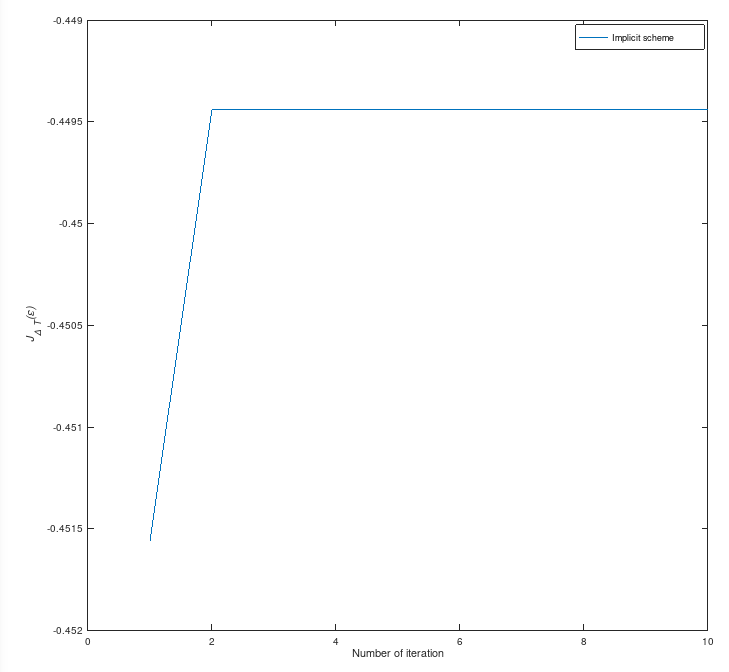
\includegraphics[scale=0.7]{images/implicit_func.png}
\end{figure}
Le schéma est bien monotone et converge de plus très rapidement.

\section{Schémas explicites}
Considérons toujours
\begin{equation}
\phi_j(\tilde{\varepsilon}_j,\varepsilon'_j) = (\tilde{\varepsilon}_j-a_j(\tilde{\varepsilon}_j,\varepsilon'_j))^2 - (\varepsilon'_j-a_j(\tilde{\varepsilon}_j,\varepsilon'_j))^2
\end{equation}
et
\begin{equation}
\tilde{\phi}_j(\varepsilon_j,\tilde{\varepsilon}_j) = (\varepsilon_j-b_{j+1}(\varepsilon_j,\tilde{\varepsilon}_j))^2 - (\tilde{\varepsilon}_j-b_{j+1}(\varepsilon_j,\tilde{\varepsilon}_j))^2
\end{equation}
Et rappelons que, étant donné la suite $(\varepsilon^{k})$:
\begin{enumerate}
	\item l'analyse de la partie négative de $\tilde{\phi}_j(\varepsilon_j^k,\tilde{\varepsilon}_j^k)$ pour chaque $j$ permet de définir la suite $(\tilde{\varepsilon}^k)$
	\item l'analyse de la partie négative de $\phi_j(\tilde{\varepsilon}_j^k,\varepsilon_j^{k+1})$ pour chaque $j$ permet de définir la suite $(\varepsilon^{k+1})$
\end{enumerate}
Sans perte de généralité travaillons sur la 2 eme étape. Considérons l'application 
$$f : x \mapsto \phi_j(\tilde{\varepsilon}_j^k,x)$$
On remarque que $f(\tilde{\varepsilon}_j^k)=\phi_j(\tilde{\varepsilon}_j^k,\tilde{\varepsilon}_j^k)0$.\\ Un choix optimal de $\varepsilon_j^{k+1}$ est $\varepsilon_j^{k+1} = argmax_{\R} f(\cdot)$. Pour determiner ce point, l'on fait le développement limité au voisinage du point $\tilde{\varepsilon}_j^k$. Posons $h=x-\tilde{\varepsilon}_j^k$ et calculons
\begin{align*}
a_j^k(\tilde{\varepsilon}_j^k,\tilde{\varepsilon}_j^k+h)
&=-\frac{1}{\alpha} \Im \langle \tilde{\chi}_j^k |\mu^{*}(\tilde{\varepsilon}_j^k,\tilde{\varepsilon}_j^k+h)| \breve{\psi}_j^{k+1} \rangle\\
&=-\frac{1}{\alpha} \Im \langle \tilde{\chi}_j^k |\mu| \breve{\psi}_j^{k+1} \rangle\\
&\quad -h\frac{\Delta T}{2\alpha} \Im \langle \tilde{\chi}_j^k |\mu^2| \breve{\psi}_j^{k+1} \rangle\\
&\quad +h^2\frac{\Delta T^2}{6\alpha} \Im \langle \tilde{\chi}_j^k |\mu^3| \breve{\psi}_j^{k+1} \rangle + o(h^2)\\
\end{align*}
Posons :
\begin{equation}
\varepsilon_0=-\frac{1}{\alpha} \Im \langle \tilde{\chi}_j^k |\mu| \breve{\psi}_j^{k+1} \rangle
\end{equation}
\begin{equation}
\varepsilon_1=\frac{\Delta T}{2\alpha} \Im \langle \tilde{\chi}_j^k |\mu^2| \breve{\psi}_j^{k+1}
\end{equation}
et
\begin{equation}
\varepsilon_2=\frac{\Delta T^2}{6\alpha} \Im \langle \tilde{\chi}_j^k |\mu^3| \breve{\psi}_j^{k+1} \rangle
\end{equation}
On remplace dans $f$ :
\begin{align*}
f(\tilde{\varepsilon}_j^k+h)= (\tilde{\varepsilon}_j^k-\varepsilon_0+\varepsilon_1 h-\varepsilon_2 h^2)^2 - (\tilde{\varepsilon}_j^k+h-\varepsilon_0+\varepsilon_1 h-\varepsilon_2 h^2)^2 + o(h^2)
\end{align*}
Ce polynôme en $h$ est maximal au point
\begin{equation}
h_{max}=\dfrac{\varepsilon_0-\tilde{\varepsilon}_j^k}{2\varepsilon_1+1}
\end{equation}
Ce qui nous donne 
\begin{equation}
\varepsilon_j^{k+1}= \tilde{\varepsilon}_j^k+h_{max}
\end{equation}
Sachant que $\tilde{\varepsilon}_j^k$ a été déterminé à l'étape 1 de façon similaire.
\subsection{Résultats numériques}
Nous considérons a nouveau :
\begin{equation}
i\dot y(t)= (A+c(t)B)y(t),
\end{equation}
En dimension2, l'évolution de la fonctionnelle $J(\varepsilon)$ est
\begin{figure}[H]
	\caption{Schéma explicite - évolution de la fonctionnelle}
	\centering
	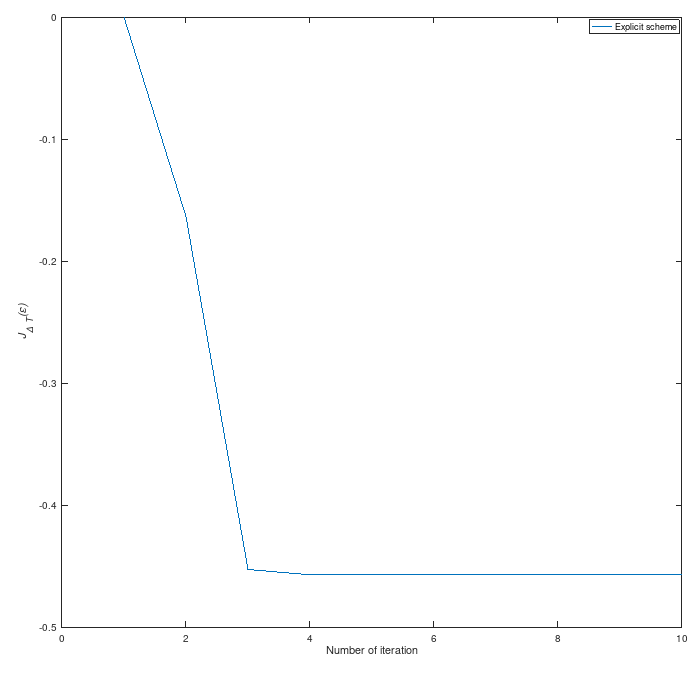
\includegraphics[scale=0.7]{images/explicit_func.png}
\end{figure}
La fonction d'onde après 10 itération de l'algorithme
\begin{figure}[H]
	\caption{Schéma explicite - évolution de la fonctionnelle}
	\centering
	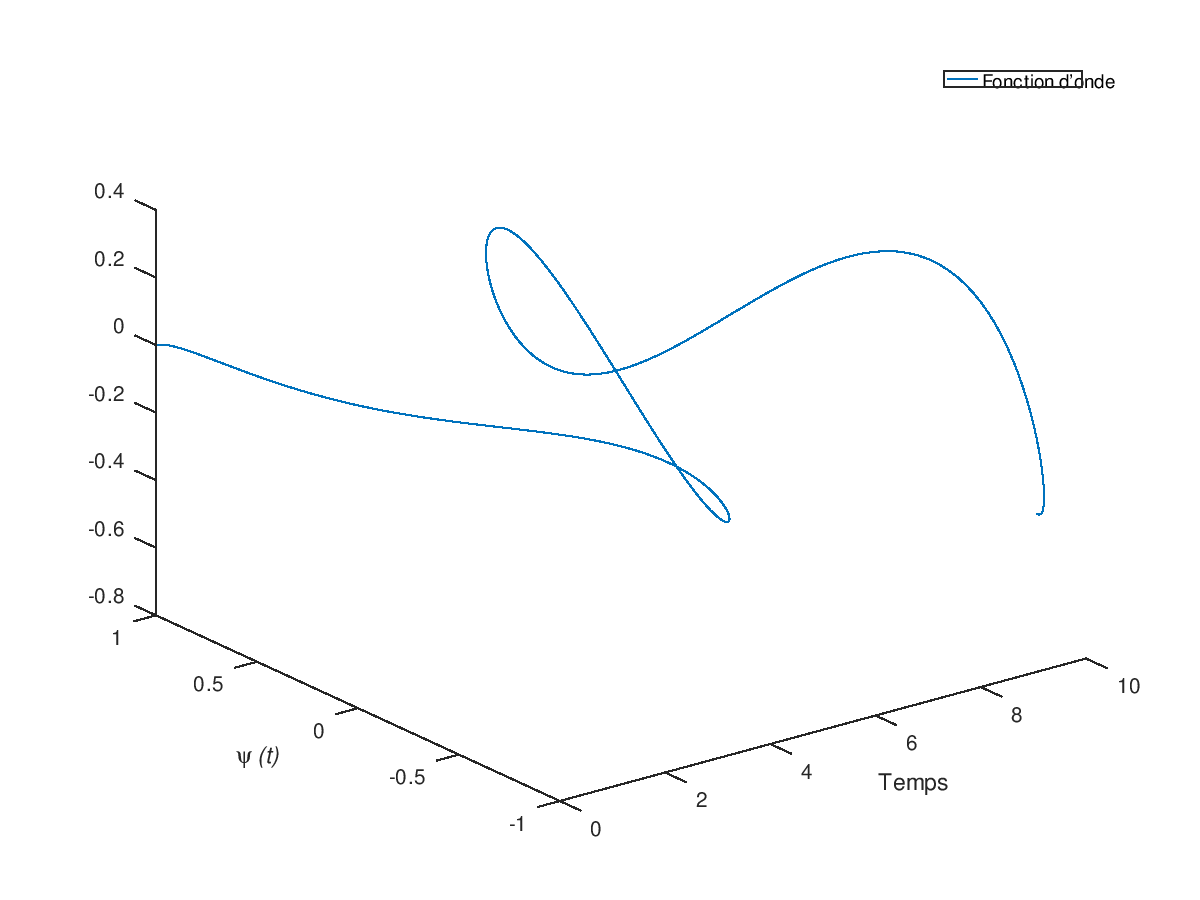
\includegraphics[scale=0.7]{images/explicit_state.png}
\end{figure}
Et enfin le contrôle obtenu
\begin{figure}[H]
	\caption{Schéma explicite - évolution de la fonctionnelle}
	\centering
	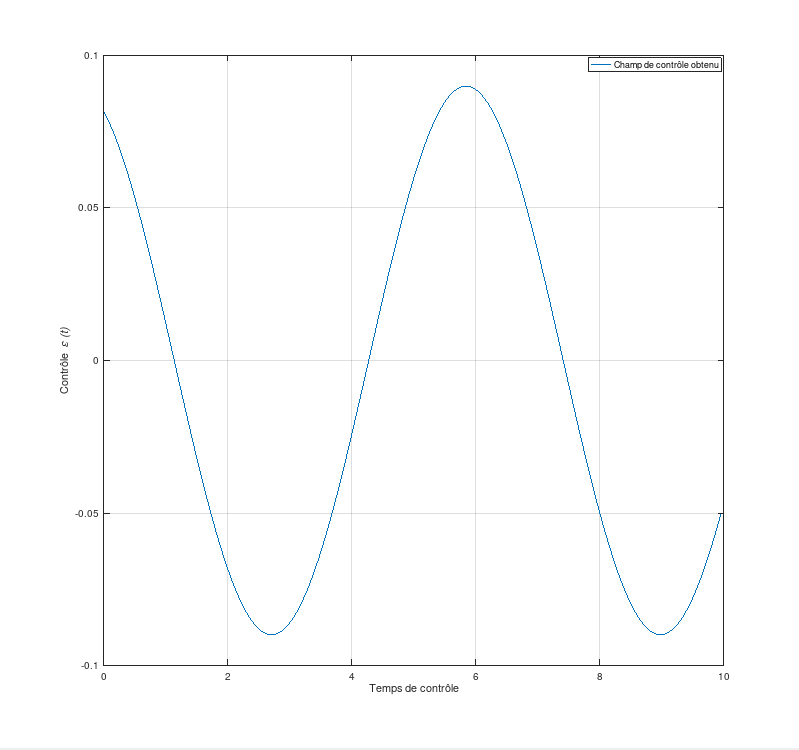
\includegraphics[scale=0.5]{images/explicit_c.png}
\end{figure}
Nous notons aussi que l'exécution du schéma explicite est très rapide par rapport a celle du schéma implicite en considérant les mêmes paramètres.\\
Pour finir, nous étudions le même problème en dimension 10, l'utilité du schéma est ici plus remarquable
\begin{figure}[H]
	\caption{Schéma explicite pour un problème en dimension 10 - évolution de la fonctionnelle}
	\centering
	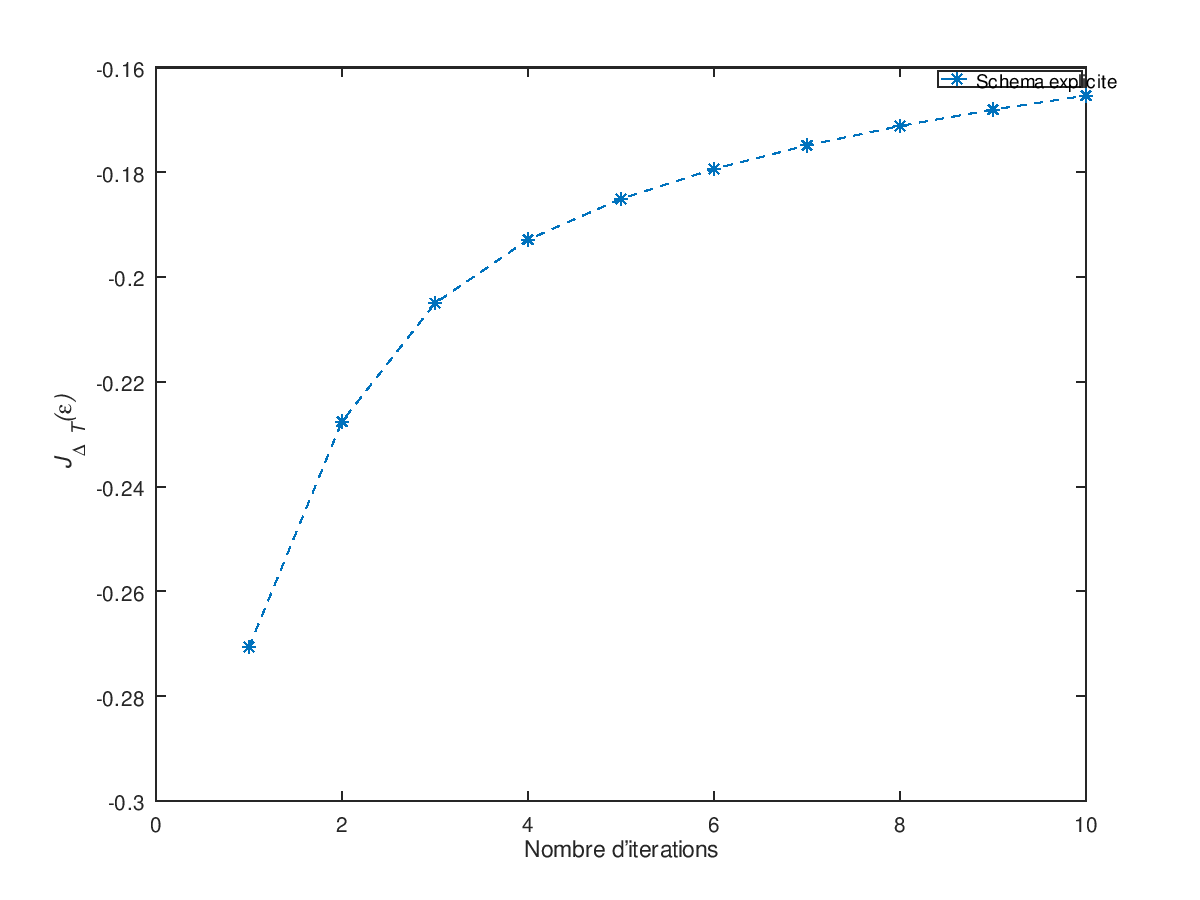
\includegraphics[scale=0.7]{images/explicitdim10_func.png}
\end{figure}